% Copyright (c) 2024, Francisco Fernandez
% License: CC BY-SA 4.0
%   https://github.com/fernandezfran/thesis/blob/main/LICENSE
\subsection{Dinámica molecular}

En la mayoría de los experimentos que se realizan en un laboratorio se obtiene 
una serie de mediciones sobre sistemas macroscópicos, usualmente constituidos por 
más de 10$^{20}$ moléculas, durante un período de tiempo, a las cuales luego se 
les realiza un promedio. La mecánica estadística ofrece una interpretación de 
las propiedades del equilibrio de sistemas macroscópicos a partir de una teoría 
molecular aplicada a su configuración microscópica ~\cite{hill1986}.

Esta teoría relaciona el promedio temporal de una variable mecánica con el 
promedio de ensambles, donde un ensamble es una colección de un número muy largo
de sistemas construidos de manera tal que reproducen las propiedades 
termodinámicas del sistema en cuestión a partir de sus configuraciones atómicas
\cite{salinas2001}. Esto es el primer postulado de la Mecánica estadística y se 
lo conoce como la \textit{hipótesis ergódica}: \say{El promedio temporal de una 
variable mecánica $M$ en el sistema termodinámico de interés es igual al promedio 
de ensambles de $M$, en el límite del conjunto de ensambles que tiende a infinito, 
siempre que los sistemas del conjunto de ensambles reproduzcan el estado 
termodinámico y el entorno del sistema real de interés}. Para poder aplicar
este postulado se necesita conocer la probabilidad relativa de cada uno de los 
estados presentes en el ensamble. A esto se refiere el segundo postulado de la 
Mecánica estadística de \textit{igual probabilidad a priori}: \say{En un conjunto 
de ensambles representativo de un sistema termodinámico aislado, los sistemas del 
conjunto de ensambles se distribuyen uniformemente, es decir, con igual 
probabilidad o frecuencia, sobre los posibles estados con los valores
especificados de dicho sistema termodinámico aislado}. En otras palabras, cada 
estado está representado por la misma cantidad de sistemas en el ensamble.

Cuando las \textit{fluctuaciones} son pequeñas, la función de distribución de 
probabilidad de la variable mecánica $M$ tiene una forma gaussiana en torno a su 
valor medio $\overline{M}$, por lo que su dispersión puede caracterizarse 
completamente por su desviación estándar $\sigma_M$, es decir,
\begin{equation}
    \sigma_M = \sqrt{\overline{(M - \overline{M})^2}}.
\end{equation}
Puede demostrarse que las \textit{fluctuaciones} de la variable mecánica $M$ 
decrecen a medida que aumenta el número de partículas $N$ presentes en el sistema 
de forma proporcional a la inversa de su raíz,
\begin{equation}\label{eq:fluctuaciones}
    \frac{\sigma_M}{\overline{M}} \approx \mathcal{O}(N^{-1/2}).
\end{equation}

Las simulaciones de Dinámica Molecular (MD, de sus siglas en inglés, 
\textit{Molecular Dynamics}) consideran un sistema clásico de muchos cuerpos 
interactuantes bajo un campo de fuerzas newtoniano para estudiar propiedades de 
equilibrio y transporte. Dada la configuración de $N$ partículas se tiene el 
siguiente sistema de ecuaciones de Newton por resolver
\begin{equation}
    m_i \frac{\partial^2 \mathbf{r}_i}{\partial t^2} = \mathbf{F}_i, \quad i = 1,..., N,
\end{equation}
donde $m_i$ es la masa del átomo $i$, $\mathbf{r}_i$ su posición y $\mathbf{F}_i$
la fuerza. Estas ecuaciones de movimiento son integradas en intervalos de tiempo
pequeños que permiten obtener la evolución temporal del sistema, es decir, su
trayectoria. Ya introducida la mecánica estadística, pueden extraerse propiedades
macroscópicas del sistema en equilibrio al considerar configuraciones microscópicas
representativas a distintos instantes de tiempo de la trayectoria
\cite{allen2017, frenkel2001}.

En la Figura \ref{fig:esquema_md} se muestra un diagrama de flujo de un algoritmo
típico de dinámica molecular para entender el funcionamiento de esta técnica de 
simulación. El mismo está conformado por las siguientes partes:
\begin{figure}[h!]
    \centering
    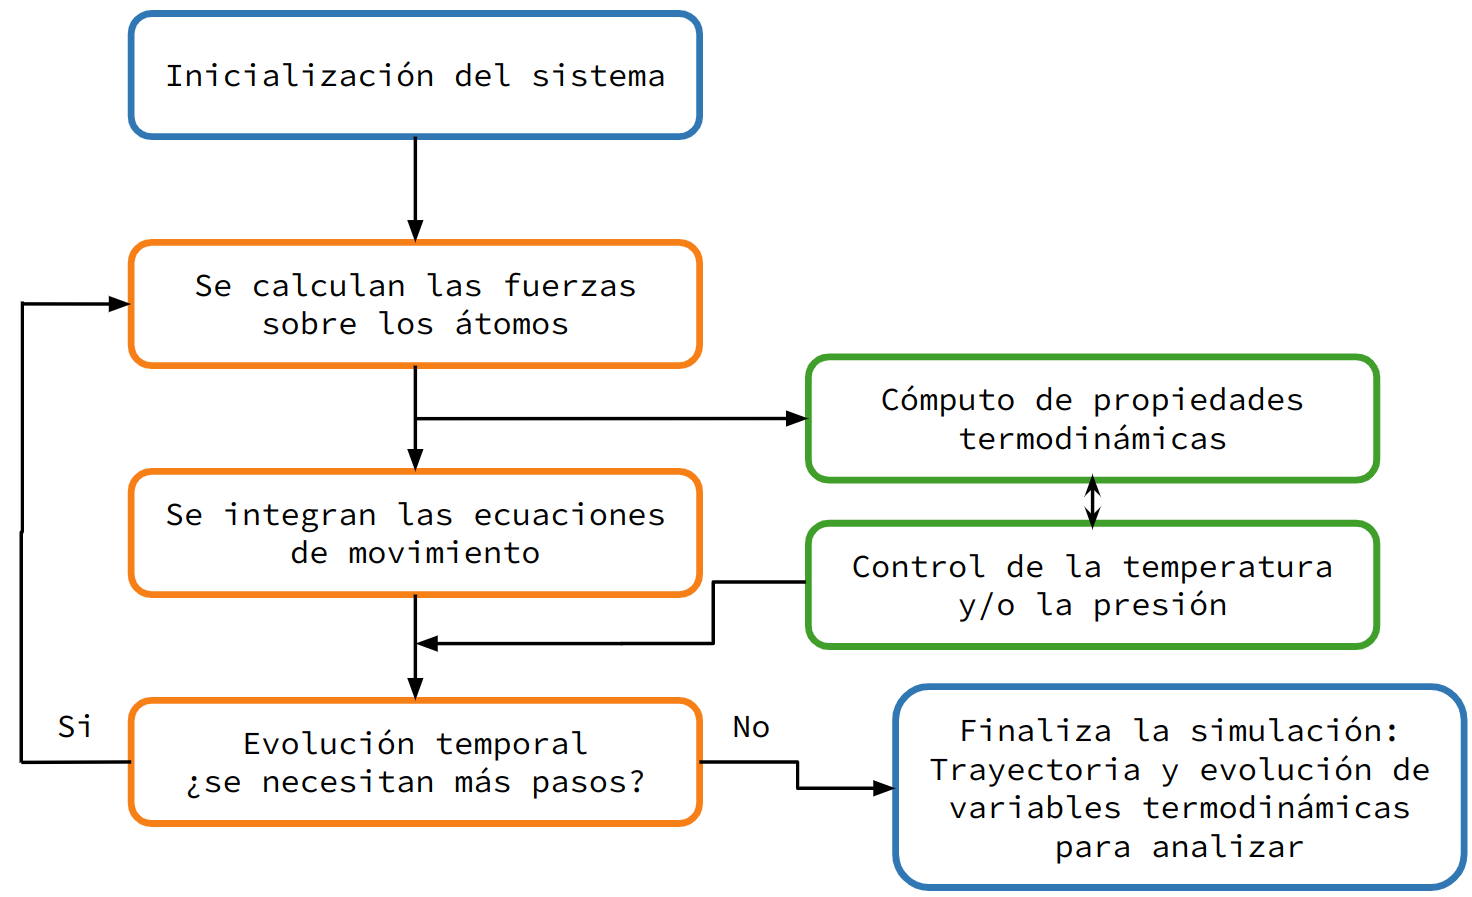
\includegraphics[width=\textwidth]{Metodos/atomicos/esquema.png}
    \caption{Esquema de un diagrama de flujo de una dinámica molecular usual.}
    \label{fig:esquema_md}
\end{figure}
\begin{enumerate}
    \item \textbf{Inicialización del sistema}: se especifican las posiciones y
        velocidades iniciales de los átomos, el tamaño y la forma de la celda de 
        simulación. También se elije un paso temporal y las condiciones de 
        contorno.
    \item \textbf{Campo de fuerzas}: con el sistema inicializado se calcula la 
        fuerza sobre cada uno de los átomos.
    \item \textbf{Cómputo de propiedades termodinámicas}: se realizan los
        cálculos de distintas cantidades de interés, como las energías potencial
        y cinética, la presión y la temperatura, etc.
    \item \textbf{Integración de las ecuaciones de movimiento}: se integran las
        ecuaciones de Newton mediante algún integrador que obtiene las posiciones
        y velocidades del paso temporal siguiente a partir del actual.
    \item \textbf{Control de la temperatura y/o la presión}: para que la 
        simulación se realice en el ensamble termodinámico deseado.
    \item \textbf{Evolución temporal}: se incrementa el tiempo adicionando un
        paso temporal y se vuelve a realizar el cálculo de las fuerzas sobre las 
        nuevas configuraciones hasta alcanzar el número de pasos temporales 
        deseados.
\end{enumerate}
Luego de este proceso se tiene la evolución temporal de las distintas propiedades
termodinámicas de interés y la trayectoria del sistema para ser analizada 
posteriormente, por ejemplo con los observables que se definirán en la sección 
\ref{s:observables}. A continuación se dan más detalles sobre cada uno de los 
pasos mencionados.


\subsubsection{Inicialización del sistema}

Existe una base de datos, Materials Project \cite{materials_project}, 
ampliamente utilizada en el ámbito académico y en la industria que 
recopila estructuras optimizadas con DFT, realiza nuevos cálculos y 
está abierta a la comunidad para su uso y colaboración. Antes de que 
los datos se carguen en la página, los mismos son comparados con resultados 
experimentales para determinar si están dentro de un rango de validez definido. 
En esta tesis en particular, se utilizaron distintas estructuras cristalinas de 
esta base de datos como condiciones iniciales para las posiciones y los tamaños 
de las celdas de simulación.

Las velocidades de los átomos suelen ser generadas de manera aleatoria, a través
de un generador de números pseudo-aleatorio, tomando como argumento una semilla 
para la reproducibilidad de la simulación y una temperatura deseada para el
sistema. Estos números son generados con una distribución gaussiana, donde el 
centro se fija a cero para que no haya una velocidad en el centro de masa y 
el ancho está relacionado a la temperatura seleccionada.

Además de dar la configuración inicial de los átomos, es necesario especificar si
los mismos se encuentran dentro de una celda de simulación, con un tamaño en
particular para cada una de las direcciones del sistema, o si
interactúan fuera
del borde de la estructura que conforman los mismos. En el primero de los casos
se tienen condiciones periódicas de contorno (PBC, por sus siglas en inglés, 
\textit{periodic boundary conditions}), que busca reproducir un sistema infinito,
para que no existan efectos de borde, y consiste en considerar que los átomos se 
encuentran dentro de una celda unidad de una red infinita de celdas idénticas; en
donde si un átomo sale por un extremo de la celda, ingresa por el opuesto.


\subsubsection{Campo de fuerzas}

Los potenciales interatómicos empíricos o semi-empíricos que usualmente se 
utilizan en las simulaciones de MD relacionan la fuerza sobre un átomo con el 
entorno del mismo a través de una forma funcional conocida. Existe una gran 
variedad de estos potenciales y la elección de uno de ellos depende del sistema 
de estudio, ya que algunos potenciales representan de mejor manera gases y otros 
metales. Por ejemplo, el potencial de Coulomb \cite{coulomb} considera las 
partículas como cargas puntuales que interactúan electrostáticamente. Los 
potenciales de Tersoff \cite{tersoff} o de Stillinger-Weber 
\cite{stillinger-weber} se desarrollaron especialmente para el modelado de 
materiales con enlaces covalentes fuertes.
El método del átomo embebido (EAM, de sus siglas en inglés) \cite{eam} 
y el EAM modificado (MEAM) \cite{meam} están diseñados para simular sistemas 
metálicos. Otros potenciales con enfoques más avanzados permiten simular
reacciones químicas en algunos sistemas, como es el caso de el COMB 
(\textit{charge-optimized many-body}) \cite{comb}, que incorpora una 
equilibración de las cargas en el modelo, o el del ReaxFF (\textit{reactive 
force fields}) \cite{reaxff}, que combina en un solo modelo distintas 
componentes de las que fueron mencionadas. En el último tiempo también se han 
desarrollado potenciales interatómicos de aprendizaje automático 
\cite{behler2016, behler2017, deringer2019}, que no tienen una forma funcional con
una interpretación física, si no más bien un mapeo entre las posiciones y la 
fuerza o la energía de un cálculo de un nivel más complejo, como puede ser DFT.

Para calcular la fuerza que actúa sobre el átomo $i$ se utiliza el opuesto 
de la derivada del potencial,
\begin{equation}\label{eq:fuerzas}
    \mathbf{F}_i = - \frac{\partial V}{\partial \mathbf{r}_i}.
\end{equation}

Para entender el comportamiento de los campos de fuerza se considera como ejemplo 
representativo el potencial de a pares de Lennard-Jones \cite{lennard-jones}, 
debido a que tiene una expresión simple de analizar,
\begin{equation}
    V_{LJ} = 4\varepsilon \left[ \left( \frac{\sigma}{r} \right)^{12} - \left( \frac{\sigma}{r} \right)^{6} \right],
\end{equation}
donde $r$ es la distancia entre dos átomos, $\varepsilon$ indica la profundidad 
del pozo del potencial que se encuentra en $r_m = 2^{1/6} \sigma$ y $\sigma$ es el
radio del átomo. En la figura \ref{fig:lj} se muestra el comportamiento de este
potencial, si la distancia entre dos átomos es menor a $r_m$ entonces se repelen,
si es mayor a dicha distancia, se atraen. Cuando la distancia entre dos átomos es 
infinita, los mismos no interactúan, en el caso práctico se define una distancia 
de corte, conocida como el \textit{radio de corte}, $r_{\text{cut}}$, a partir de 
la cual se considera que el potencial es nulo. Para evitar discontinuidades en 
este punto se suelen utilizar distintas técnicas como el truncado y desplazado o 
se multiplica al potencial alrededor de dicho punto por una función suave, que 
hace que el potencial se aproxime suavemente a cero.
\begin{figure}[h!]
    \centering
    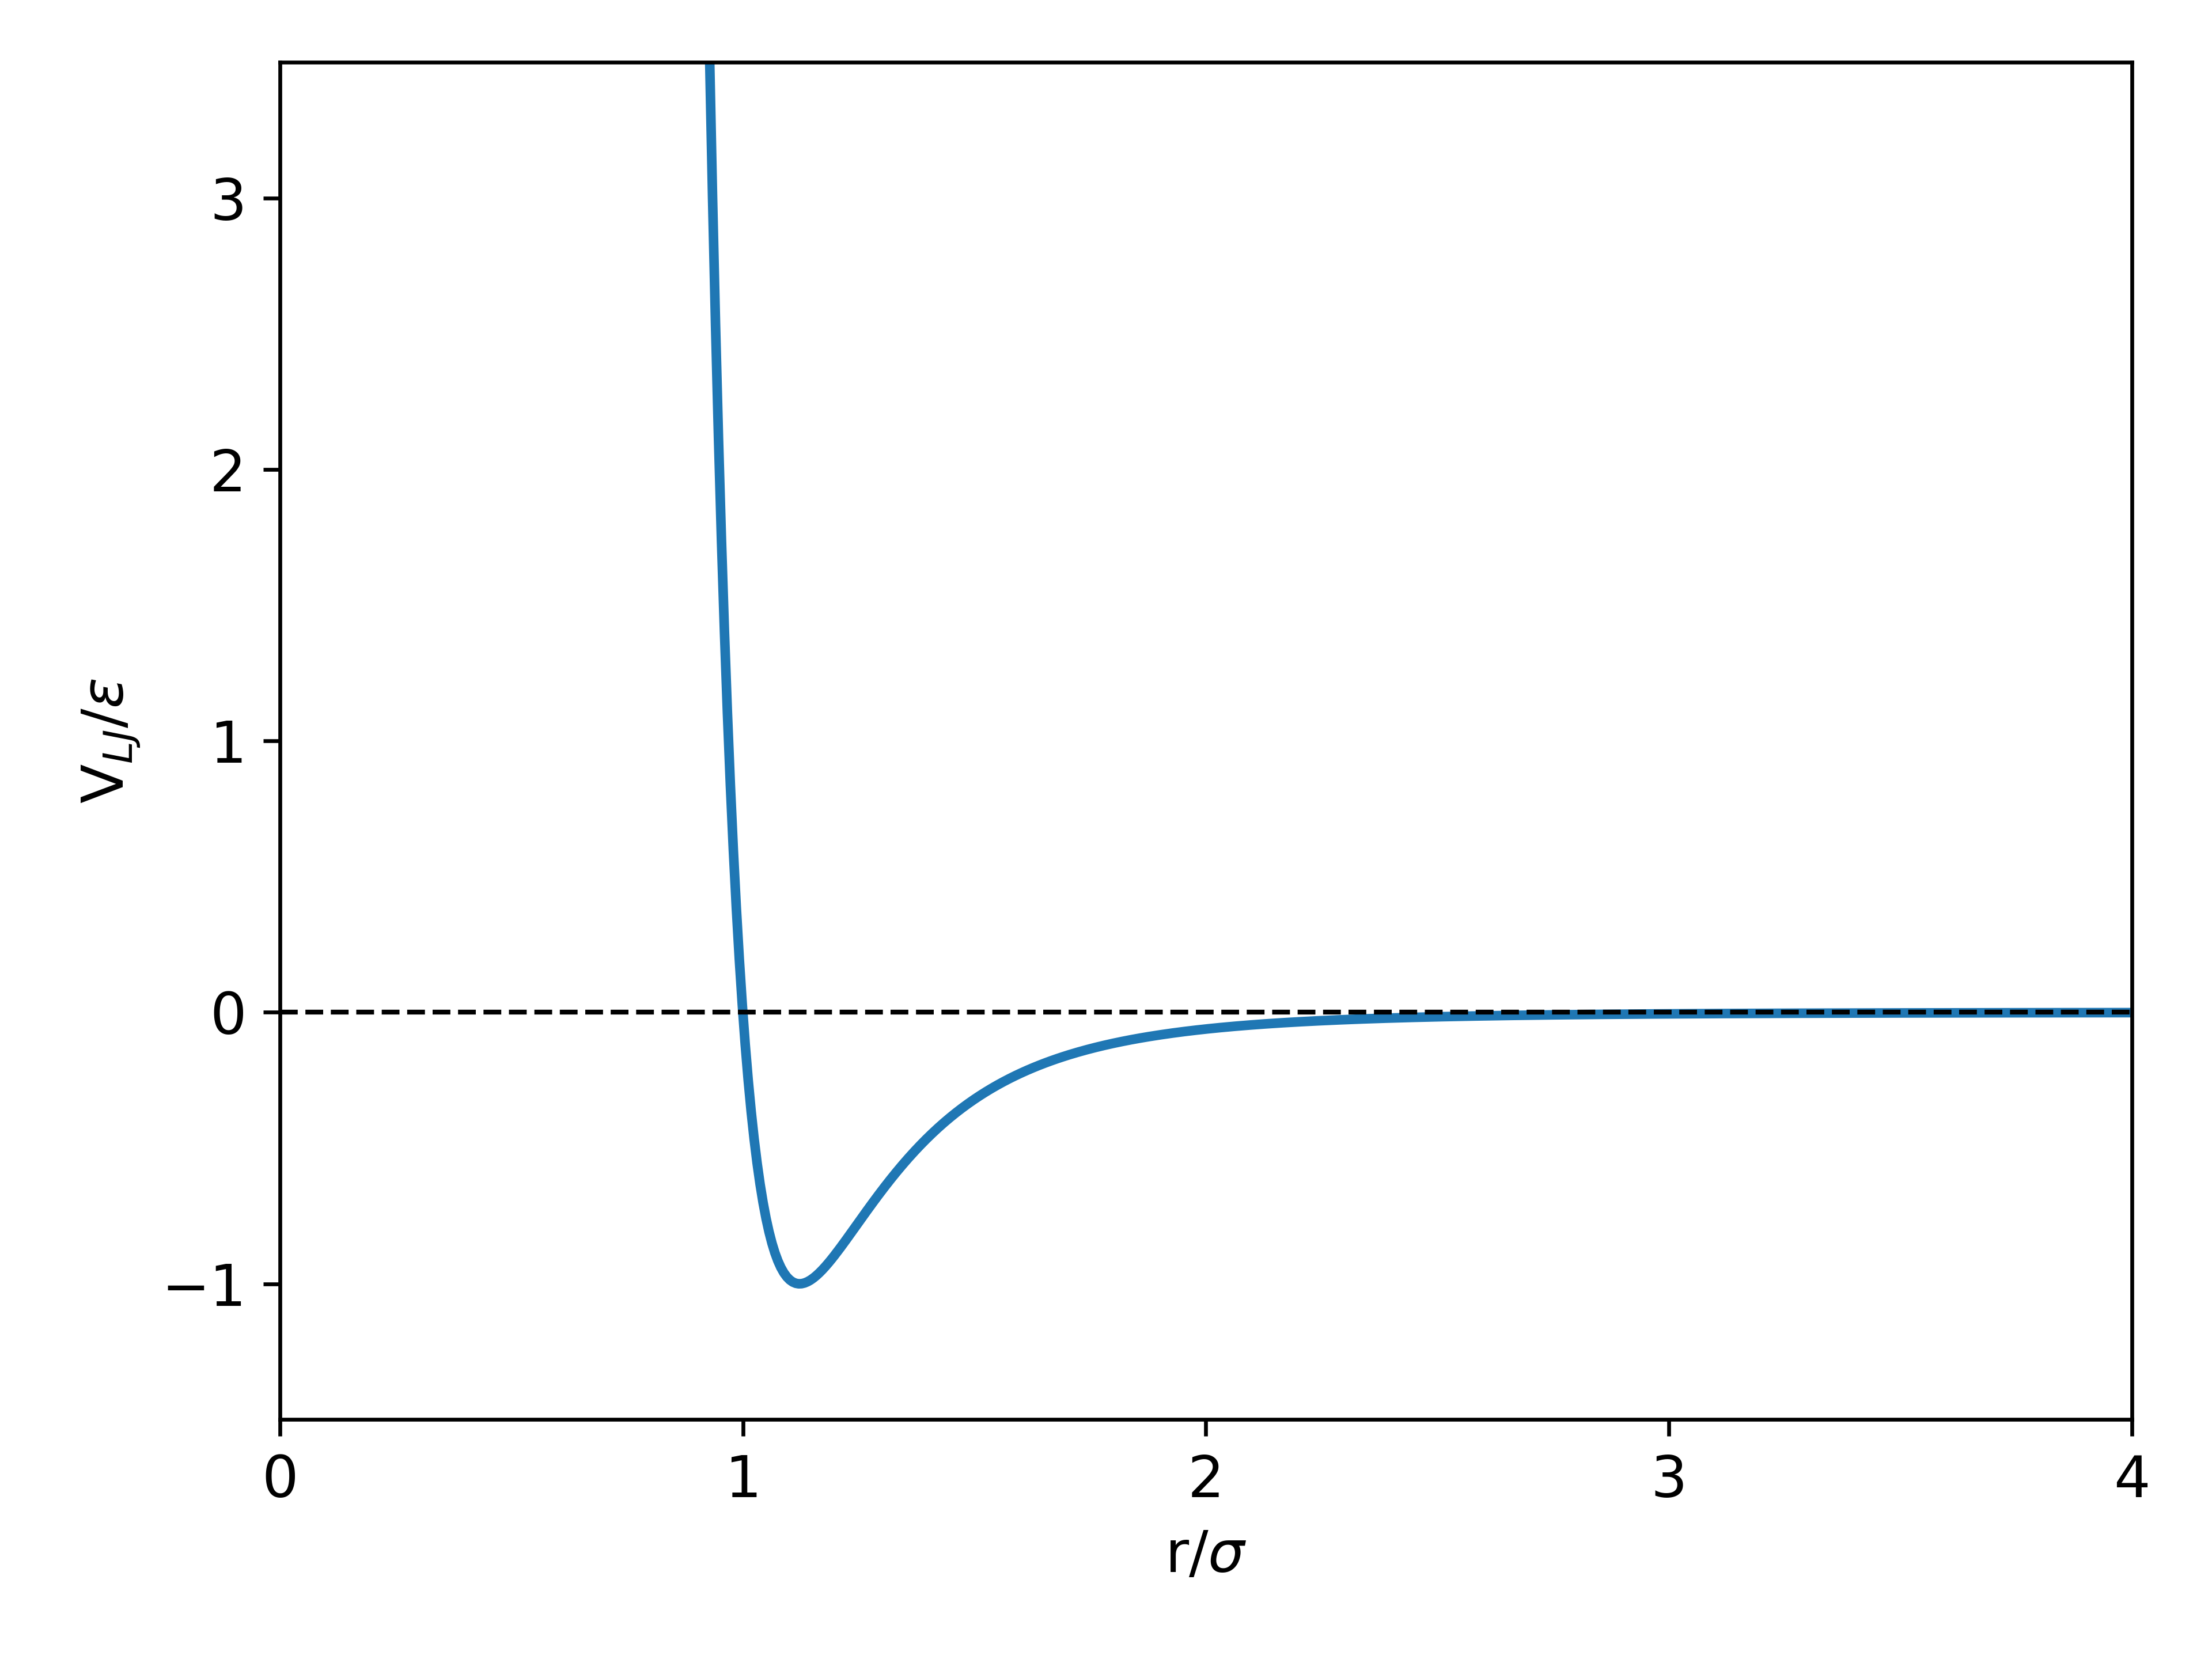
\includegraphics[width=0.7\textwidth]{Metodos/atomicos/lj.png}
    \caption{Gráfico de un potencial de Lennard-Jones en unidades reducidas.}
    \label{fig:lj}
\end{figure}

El ReaxFF \cite{reaxff} es el potencial reactivo del estado del arte para 
utilizar en simulaciones de MD de sistemas de interés en baterías de litio, ya
que representa adecuadamente la asociación y disociación de enlaces de átomos al 
considerar que la energía del sistema, $E_{\text{system}}$, se encuentra dividida
en varias contribuciones de energías parciales,
\begin{equation}\label{eq:reaxff}
    E_{\text{system}} = E_{\text{bond}} + E_{\text{over}} + E_{\text{under}} + E_{\text{val}} + E_{\text{pen}} + E_{\text{tors}} + E_{\text{conj}} + E_{\text{vdWaals}} + E_{\text{Coulomb}}.
\end{equation}
Una de las suposiciones fundamentales del ReaxFF es que el orden de enlace entre
un par de átomos puede obtenerse directamente de la distancia que los separa, 
esto se asegura con el término $E_{\text{bond}}$. $E_{\text{over}}$ y 
$E_{\text{under}}$ se agregan para imponer penalidades a los átomos 
sobrecoordinados o subcoordinados, utilizando la teoría de la valencia del enlace.
$E_{\text{val}}$ considera la contribución a la energía por el ángulo de valencia, 
mientras que $E_{\text{pen}}$ penaliza sistemas para reproducir la estabilidad de 
sistemas con dos dobles enlaces que comparten un átomo en un ángulo de valencia.
Las contribuciones a la energía de los ángulos de torsión y de los efectos de 
conjugación están dados por $E_{\text{tors}}$ y $E_{\text{conj}}$, 
respectivamente. Por último, las interacciones repulsivas a distancias 
interatómicas cortas y las atractivas a distancias largas son incluidas para 
todos los pares de átomos mediante un término de van der Waals, 
$E_{\text{vdWaals}}$, utilizando un potencial de Morse, y uno de Coulomb, 
$E_{\text{Coulomb}}$, donde las cargas de los átomos se aproximan a través de 
un método de equilibración.

La expresión dada en la ecuación \ref{eq:reaxff} implica una gran cantidad de 
parámetros ajustables que se obtienen a partir de cálculos de química cuántica
sobre la disociación de enlaces, reacciones de moléculas pequeñas, energías de 
formación y geometrías de distintos compuestos. Una parametrización ya existente
para el sistema Li-Si \cite{fan2013} se utiliza en el capítulo 
\ref{ch:caracterizacion}.

En los capítulos \ref{ch:modelo} y \ref{ch:prediccion} se utiliza un enfoque 
híbrido que consiste en considerar el hamiltoniano del método DFTB, introducido 
en la sección \ref{s:dftb}, en la ecuación \ref{eq:fuerzas} para calcular las 
fuerzas en una dinámica molecular.


\subsubsection{Cómputo de propiedades termodinámicas}

Una vez que ya se conocen las posiciones, velocidades y fuerzas de todos los 
átomos, se tiene toda la información necesaria para computar distintas cantidades 
de interés. Por ejemplo, para el cálculo de la energía total ($E_{\text{tot}}$) 
se tiene la suma de la contribución potencial ($E_{\text{pot}}$) y de la cinética
($E_{\text{cin}}$),
\begin{equation}
    E_{\text{tot}} = E_{\text{pot}} + E_{\text{cin}}.
\end{equation}
La primera de ellas viene dada por 
\begin{equation}
    E_{\text{pot}} = \sum_{i < j} u(\mathbf{r}_{ij}),
\end{equation}
donde $u(\mathbf{r}_{ij})$ es la contribución proveniente de la interacción 
entre los átomos $i$ y $j$. Por otro lado, la energía cinética puede calcularse a
partir de las velocidades de cada uno de los átomos como
\begin{equation}
    E_{\text{cin}} = \frac{1}{2} \sum_{i=1}^{N} m_i v_i^2, 
\end{equation}
donde $m_i$ es la masa del átomo $i$ y $v_i^2$ el módulo de su velocidad. 

También suele ser de interés obtener el valor de la temperatura y de la presión
del sistema. La temperatura en un paso de la simulación puede calcularse 
utilizando que
\begin{equation}\label{eq:tempvel}
    k_B T = \sum_{i=1}^N \frac{m_i v_i^2}{N_f},
\end{equation}
donde $k_B$ es la constante del Boltzmann y $N_f$ los grados de libertad,
aproximados usualmente por $3N$ para sistemas lo suficientemente grandes. Por 
último, la presión puede calcularse como 
\begin{equation}
P = \rho k_B T + \frac{1}{d \cdot V} \left\langle \sum_{i<j} \mathbf{f}(\mathbf{r}_{ij}) \cdot \mathbf{r}_{ij} \right\rangle,
\end{equation}
donde $\rho$ es la densidad, $d$ la dimensión y $V$ el volumen de la celda de 
simulación. El segundo término es conocido como el virial, donde $\mathbf{r}_{ij}$ 
y $\mathbf{f}(\mathbf{r}_{ij})$ son las distancias y las fuerzas entre los átomos $i$ y $j$.


\subsubsection{Integración de las ecuaciones de movimiento}

Para la integración de las ecuaciones de movimiento se utiliza un integrador que 
cumple con la función de evolucionar las velocidades y las posiciones de los 
átomos una vez que ya se conocen las fuerzas aplicadas sobre cada uno de ellos.
Un integrador estándar, utilizado en esta tesis, es el \textit{velocity Verlet}. 
Para las posiciones se tiene una actualización de las mismas, a partir
del paso actual, como un desarrollo de Taylor de orden 2,
\begin{equation}
    r(t+dt) = r(t) + v(t) dt + \frac{f(t)}{2m} dt^2,
\end{equation}
donde $dt$ es el paso temporal y $m$ la masa del átomo. Para las velocidades se
tiene
\begin{equation}
    v(t+dt) = v(t) + \frac{f(t+dt)+f(t)}{2m} dt,
\end{equation}
es importante notar que para calcular la velocidad del paso temporal siguiente se
necesita tener computadas las fuerzas anteriores y posteriores, por lo cual
primero se calculan las posiciones y, a partir de ellas, las fuerzas y recién 
luego las velocidades. 


\subsubsection{Control de la temperatura y/o la presión}

Debido a que la dinámica molecular usual se realiza en un ensamble con el número 
de partículas, el volumen y la energía total constantes (NVE) y la mayoría de los
experimentos con los cuales se pueden comparar resultados se llevan a cabo en 
condiciones de temperatura y/o presión constante, es necesario introducir 
distintos termostatos y barostatos que permitan controlar estos parámetros en las 
simulaciones realizadas. Para modelar el comportamiento directamente de estados
de equilibrio en estos ensambles, se puede modificar la dinámica molecular. 

Desde el punto de vista de la mecánica estadística, a un sistema se le puede 
imponer una temperatura (ensamble NVT) si se lo pone en contacto con un baño 
térmico lo suficientemente grande. En dicho caso la probabilidad de encontrar al 
sistema en un estado de energía viene dada por la distribución de 
Maxwell-Boltzmann,
\begin{equation}\label{eq:mb}
    P(p) = \left( \frac{\beta}{2\pi m} \right)^{3/2} exp(-\beta p^2 / (2m)),
\end{equation}
donde $\beta$ es la energía térmica $1 / (k_B T)$. Esto quiere decir que la velocidad 
de un átomo no se mantiene constante cuando está en contacto con un baño térmico, 
sino que la misma puede fluctuar y la fluctuación va a depender de dicha 
temperatura de la siguiente forma
\begin{equation}
    \sigma_T^2 = \frac{2}{3 N} \langle T \rangle_{NVT}^2,
\end{equation}
que proviene de calcular el segundo y el cuarto momento de la ecuación 
\ref{eq:mb}.

De manera análoga se puede dejar de suponer al volumen como constante y empezar a
pensar que el mismo es una variable, acoplando el sistema a un pistón para tener
una presión deseada (NPT).

Distintos termostatos y barostatos fueron utilizados durante esta tesis, ellos 
son: el termostato y barostato de Berendsen \cite{berendsen1984}, el termostato 
de Langevin \cite{schneider1978, kroger2005}, el termostato de Nosé-Hoover 
\cite{nose1984a, nose1984b, hoover1985} y el barostato de Parrinello-Rahman
\cite{parrinello-rahman}.
